\documentclass[a4paper,12pt]{article}
\usepackage[utf8]{inputenc}
\usepackage[cm,empty]{fullpage}
\usepackage[T2A]{fontenc}
\usepackage[english, russian]{babel}
\usepackage{amssymb,amsmath,amsxtra,amsthm}
\usepackage{proof}
\usepackage[pdftex]{graphicx}
\usepackage{wrapfig}
\usepackage{braket}
\usepackage{xcolor}

\usepackage[left=2cm,right=2cm,
    top=1cm,bottom=1cm,bindingoffset=0cm]{geometry}

\renewcommand{\leq}{\leqslant}
\renewcommand{\geq}{\geqslant}


\newcommand{\iiff}{\Longleftrightarrow}
\renewcommand{\iff}{\Leftrightarrow}
\newcommand{\nothing}{\varnothing}

\newtheorem*{rem}{Замечание}

\newcommand{\NN}{\mathbb{N}}
\newcommand{\ZZ}{\mathbb{Z}}
\newcommand{\Q}{\mathbb{Q}}
\newcommand{\A}{\mathbb{A}}
\newcommand{\R}{\mathbb{R}}
\renewcommand{\C}{\mathbb{C}}

\renewcommand{\phi}{\varphi}
\newcommand{\eps}{\varepsilon}

\newcounter{z}


\newcommand{\zs}{\refstepcounter{z}\vskip 10pt\par\noindent
\fbox{\textbf{12.\arabic{z}}} }

\newcommand{\z}{\refstepcounter{z}\vskip 20pt\noindent
\fbox{\textbf{\arabic{z}}} }

\renewcommand{\date}{{\bf 7 февраля 2021}} %Дата занятия

\newcommand{\dif}
{
------------------------------------------------------------------------------------------------------------------------------------------------------
}

\newcommand{\HSEhat}{
\vspace*{-0pt}
\noindent
\setcounter{z}{0}


{\bf \phantom{\date}  \large \hfill Дискретная математика: \hfill \normalsize \date}

\vspace{5 pt}
{\bf \large \hfill  ориентированные графы и алгоритмы на графах.\hfill }

\vspace{15 pt}
\centerline{ \large  Домашнее задание.}
\centerline{ \large  Кирилл Сетдеков}



\vspace*{10pt}
\setcounter{z}{0}

}

\begin{document}

\HSEhat



\centerline{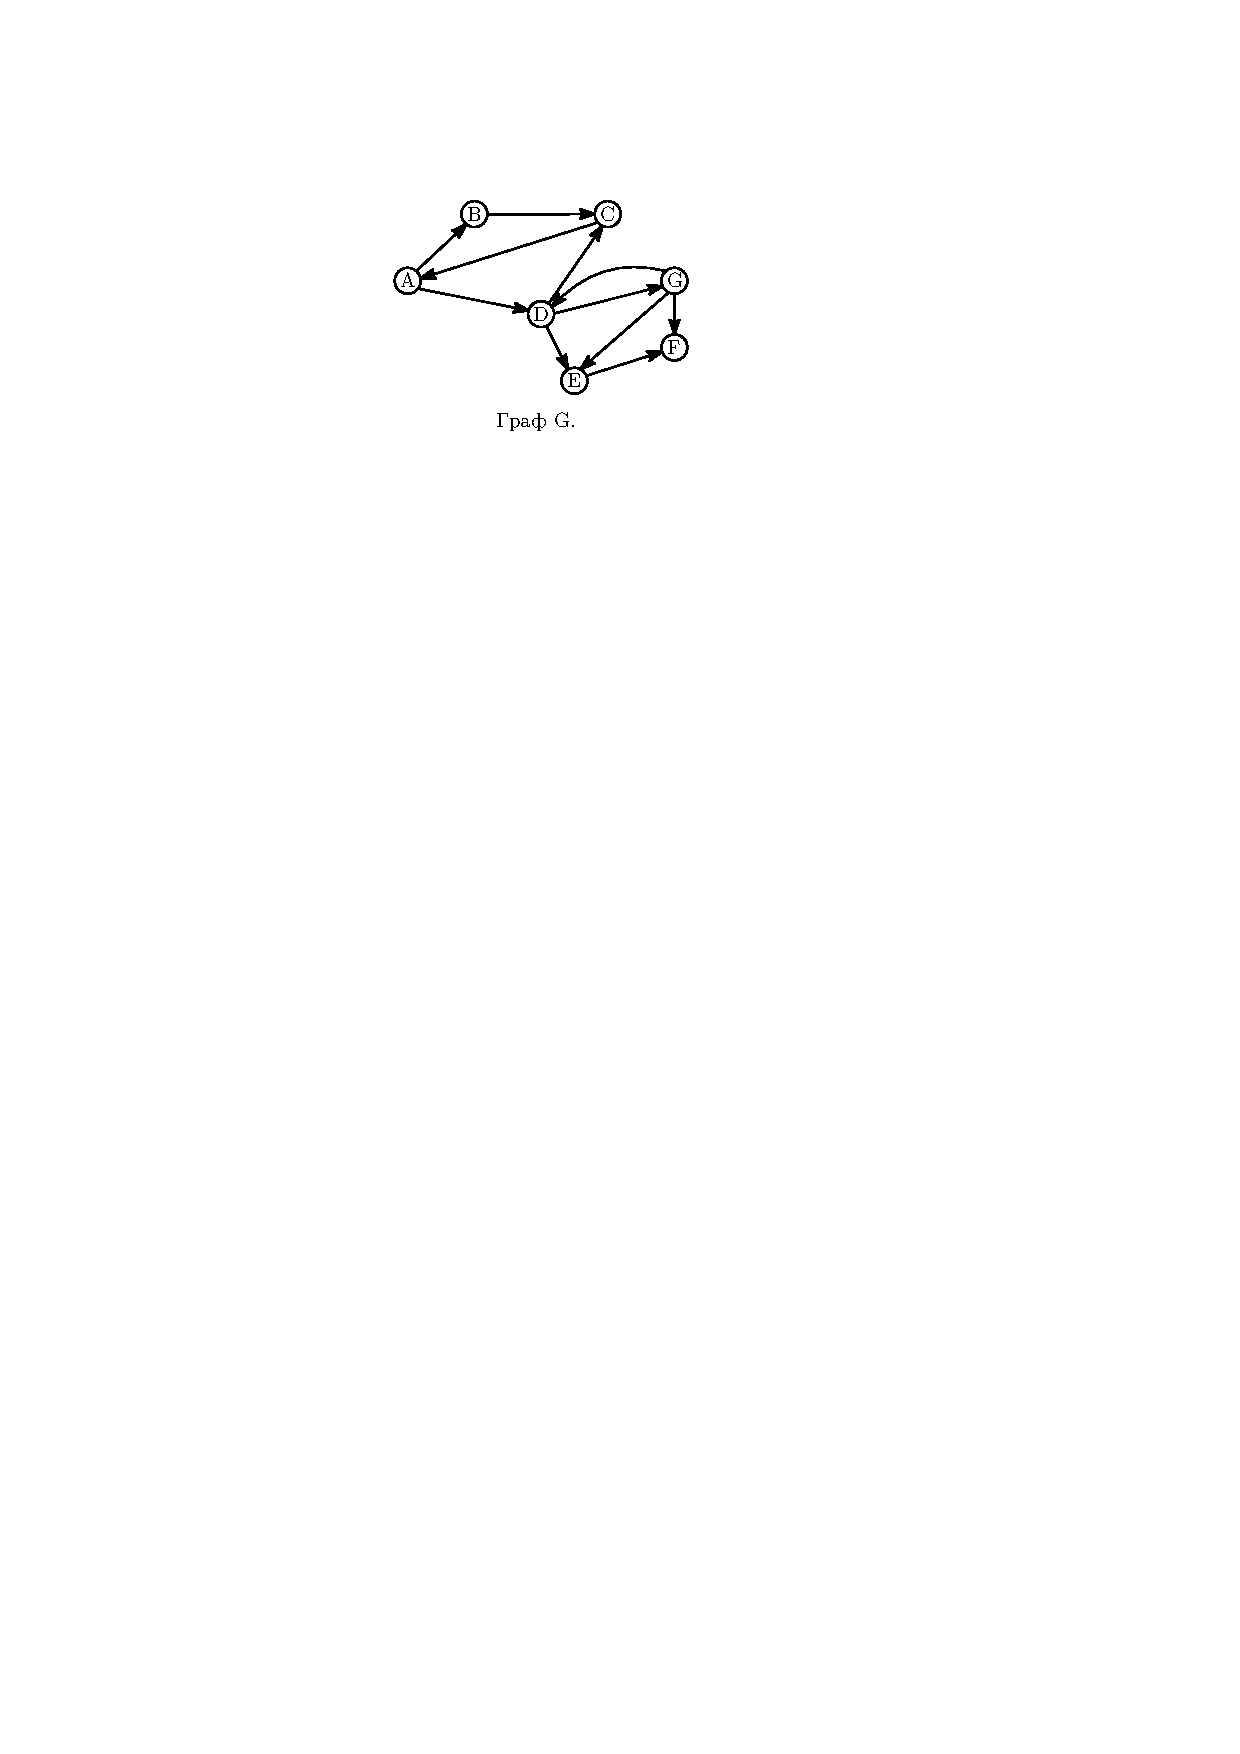
\includegraphics[scale=1.1]{img/digraphHW.pdf}\qquad \qquad 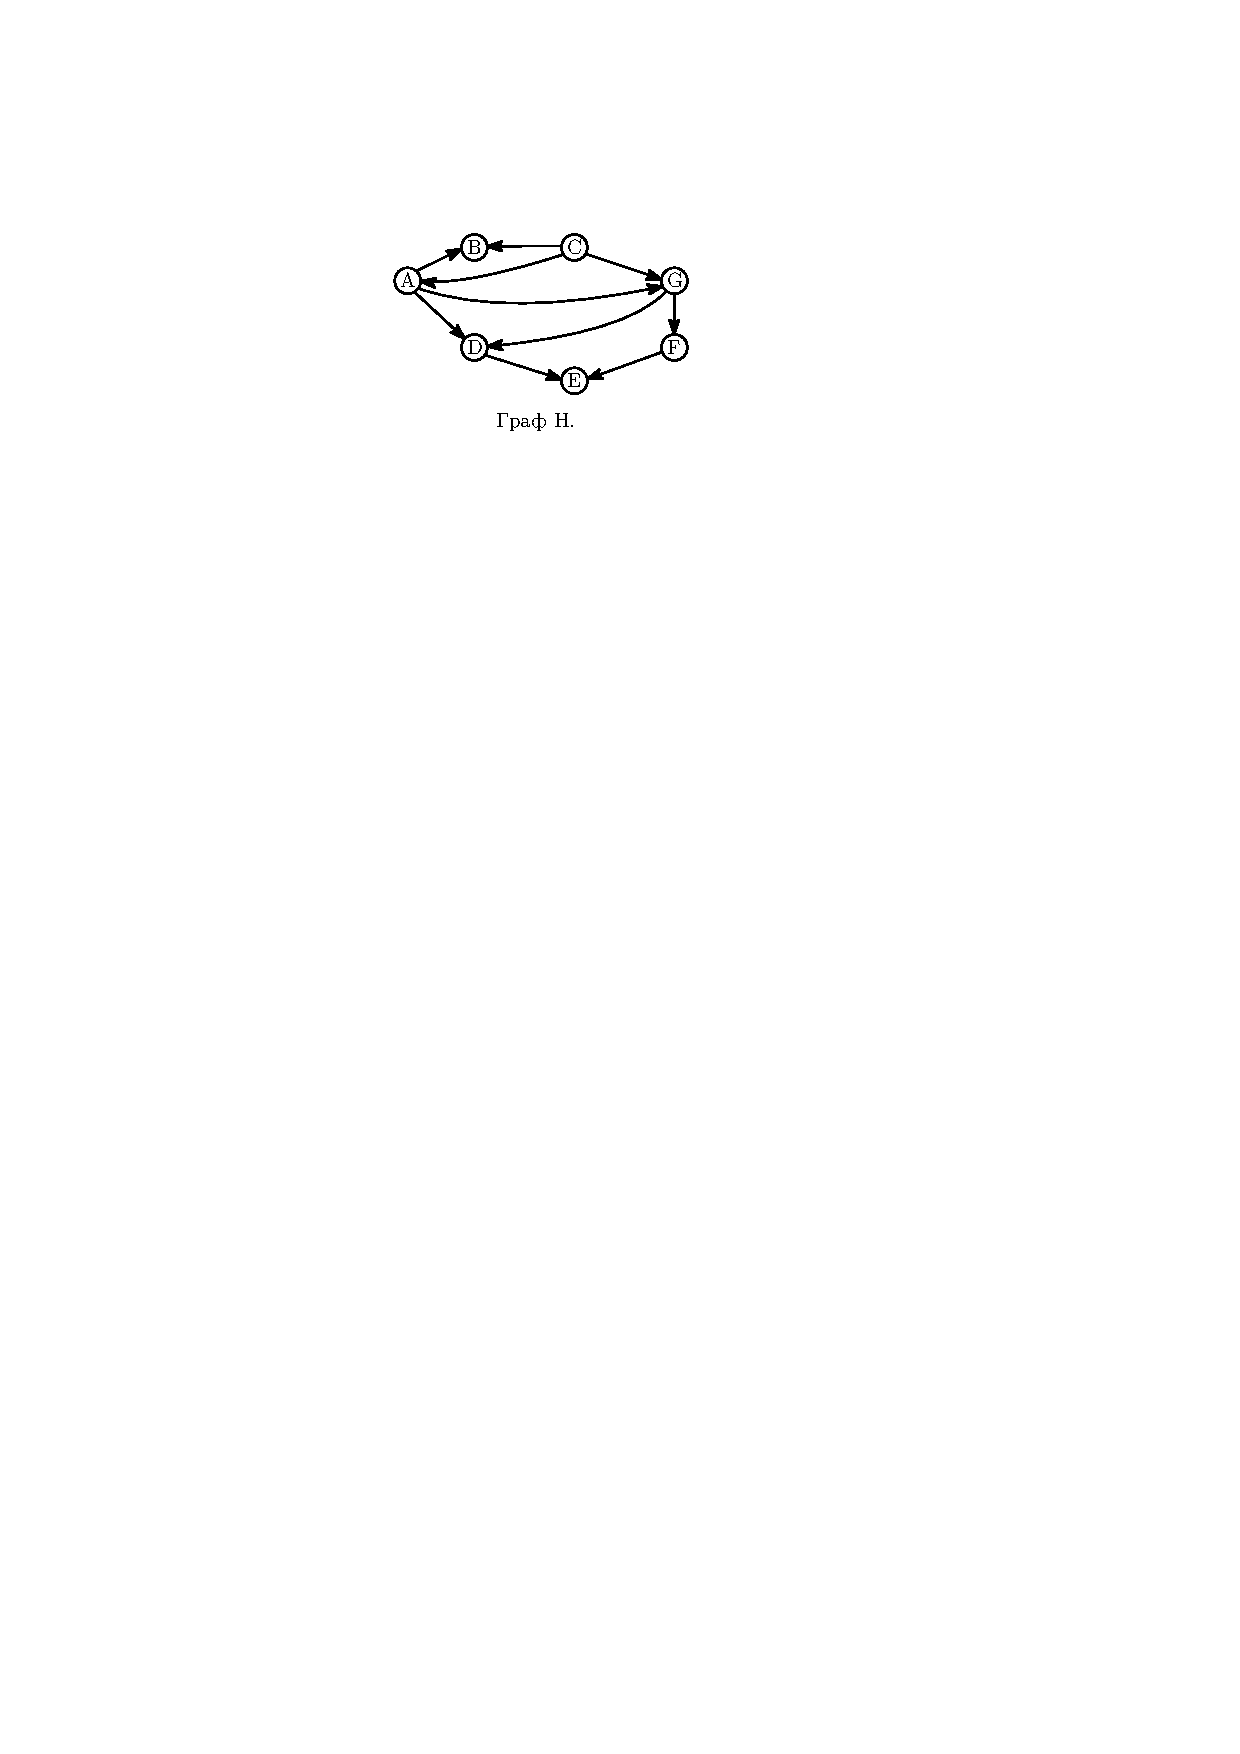
\includegraphics[scale=1.1]{img/digraphHW2.pdf}}

\z Граф $G$ изображен на рисунке выше.\\
{\bf a)} Найдите максимальную длину простого цикла в графе $G$. Укажите
все различные простые циклы максимальной длины. (Достаточно предъявить ответ)\\

\textbf{Ответ: Максимальная длина простого цикла в графе $G$ = 3. Есть два простых цикла в этом графе: $(A,B,C,A)$ и $(A,D,C,A)$}

{\bf б)} Найдите компоненты сильной связности графа $G$. (Достаточно предъявить ответ)\\
\textbf{Ответ: В этом графе есть 3 компоненты сильной связности: $\set{A,B,C,D,G}$ ; $\set{E}$ ; $\set{F}$}

{\bf в)} Какое минимальное число рёбер необходимо добавить в граф $G$, чтобы
он стал сильно связным? (Необходимо обоснование ответа)

\textbf{Решение:} \\
Сейчас граф не является сильно связанным, так как есть вершина $F$ из которой нельзя добраться в другие.

Проверим для числа добавляемых ребер = 1.

Если мы сможем найти такие две вершины, так что после добавления ребра, вершина $E$ и $F$ будут достижимы из компоненты связности $\set{A,B,C,D,G}$ и наоборот, тогда мы получим граф с одной компонентой связности.

Проверим новое ребро $(F,D)$.

Вместе с ним получается простой цикл $(D,E,F,D)$. Вершины $E$ и $F$ входят в этот цикл $\Rightarrow$ входят в одну компоненту связности. При этом их этого цикла можно попасть в компоненту связности $\set{A,B,C,D,G}$ и наоборот $\Rightarrow$ в графе теперь одна компонента связности $\Rightarrow$ граф стал сильно связным после добавление 1 ребра

\textbf{Ответ:1 ребро, например $(F,D)$}
\z Ациклический граф $H$ изображен на рисунке выше. Осуществите топологическую сортировку вершин графа $H$.
(Достаточно предъявить ответ. В ответе можно, например, указать последовательность вершин от меньшего номера к большему.)

\textbf{Ответ: нумерация вершин, используя поиск в глубину, так что ребро ведет от меньшего номер вершины к большему. Каждой вершине сопоставлен номер: $\set{(C,1), (A,2), (B,3), (G,4), (D,5), (F,6), (E,7)}$}

\vskip 10 pt

{\it К остальным задачам необходимо привести решения с обоснованием.}

\vskip 10 pt
\centerline{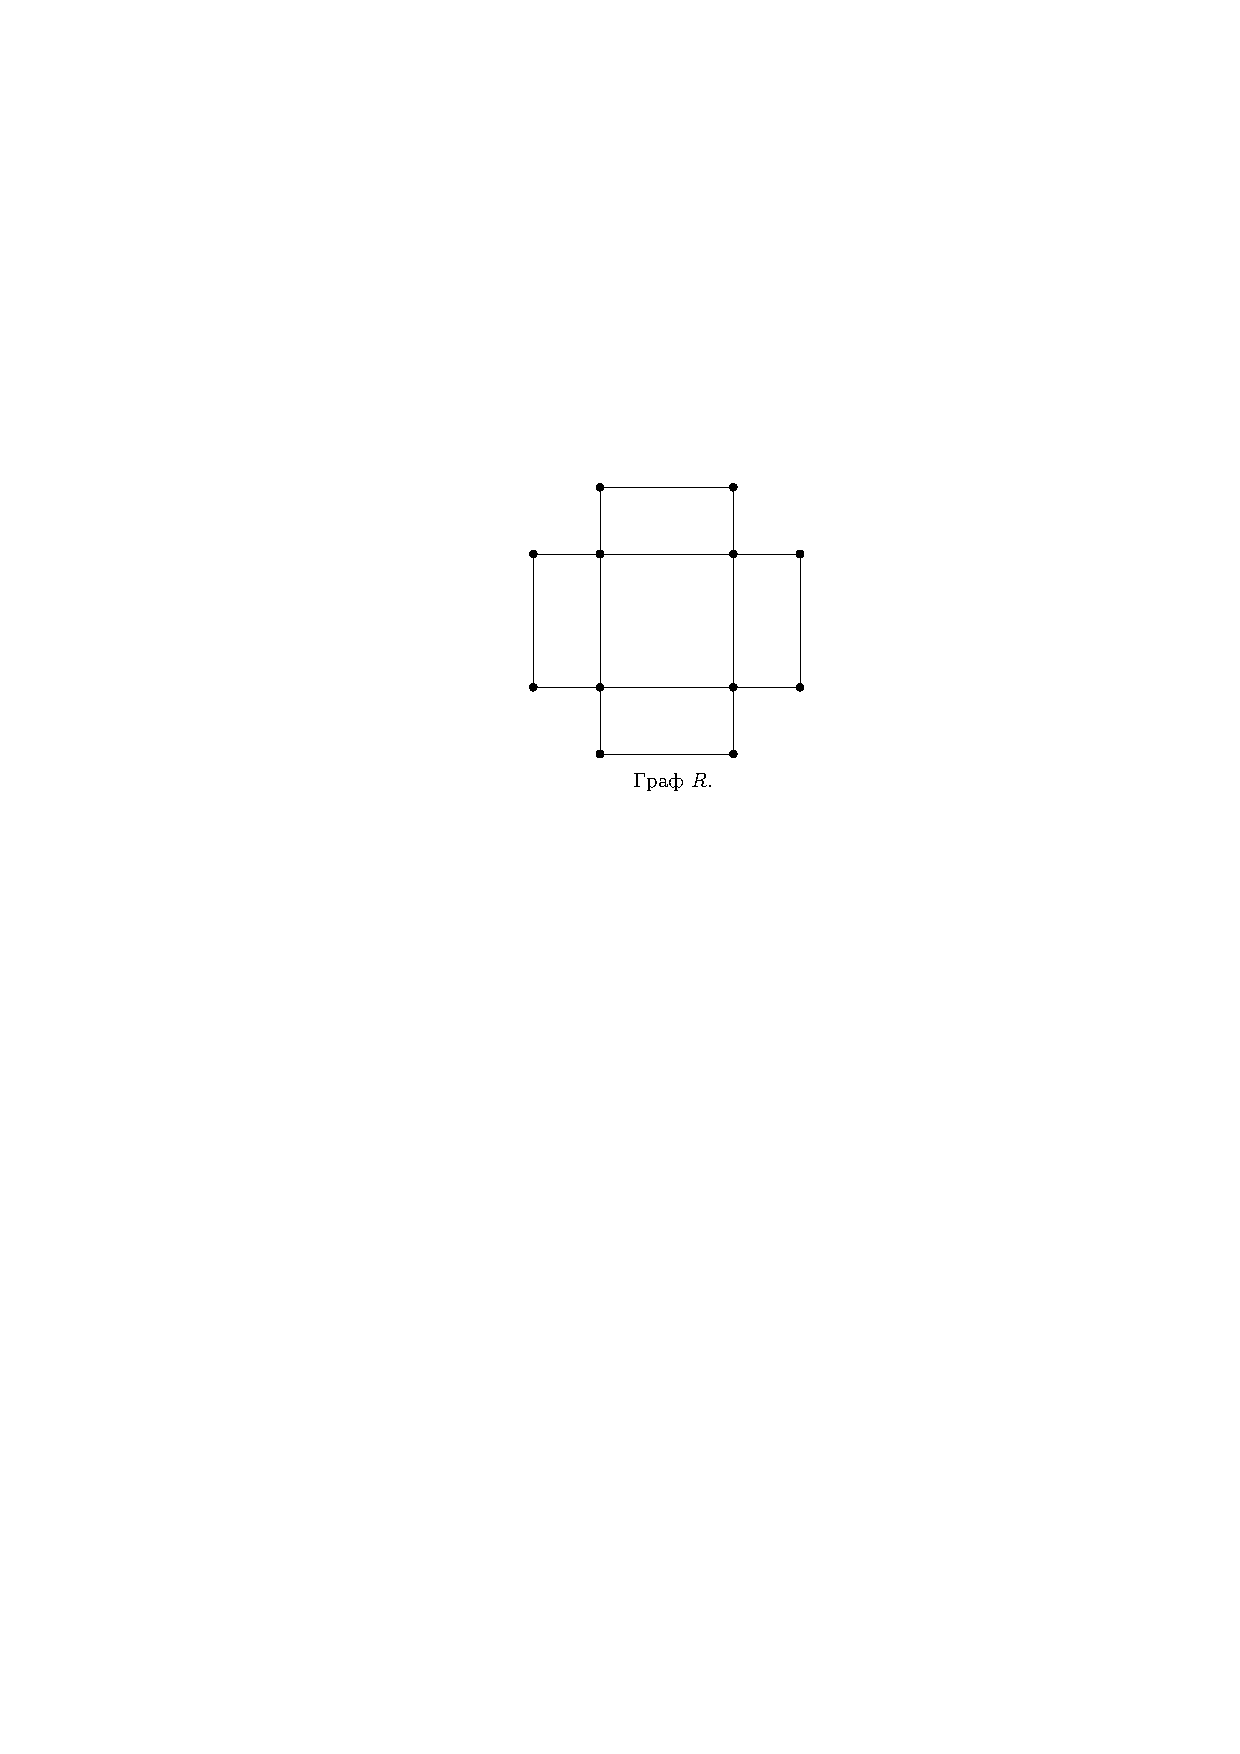
\includegraphics[scale=1.1]{img/HgraphHW.pdf}}

\z Граф $R$ изображен на рисунке выше. Верно ли, что граф $L(R)$ гамильтонов?

\textbf{Решение:} \\
Нарисуем $L(R)$

\centerline{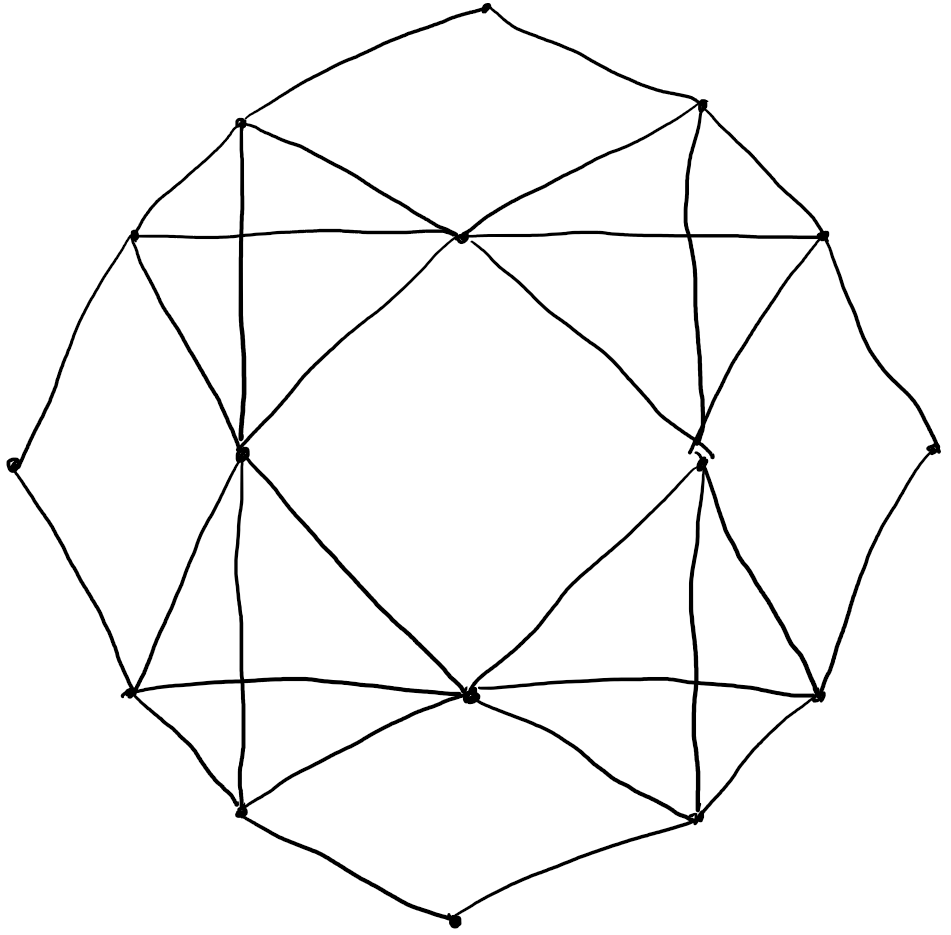
\includegraphics[width=0.33\textwidth]{img/Lg.png}}

На основании доказанной теоремы "Если $R$ имеет эйлеров цикл, то $L(R)$ имеет как эйлеров, так и гамильтонов циклы", нам достаточно доказать что в графе $R$ есть эйлеров цикл.

В графе $R$ все вершины имеют степень 2 или 4.
$${deg(v_i)} \in \set{2,4}$$ 
$\Rightarrow$ все вершины имеют четную степень $\Rightarrow$ $R$ имеет эйлеров цикл $\Rightarrow$ $L(R)$ имеет гамильтонов цикл


\textbf{Ответ: Граф $L(R)$ имеет гамильтонов цикл согласно решению выше.}

\z На плоскости отмечено $15$ точек, которые соединены $25$ непересекающимися отрезками так, что от любой точки можно добраться до любой другой по 
этим отрезкам.\\
{\bf а)} На сколько частей разбита плоскость этой фигурой?\\
\textbf{Решение:} \\
Из условия фигура нарисована на плоскости $\Rightarrow$ это нарисован планарный граф.

Для планарного графа выполняется $$|V| - |E| +|F| = 2$$, где $|V| = 15$ - число вершин, $|E| = 25$ - число ребер, $|G|$ - число граней на плоскости.

$$25 - 15 +|F| = 2$$
$$|F| = 12$$

\textbf{Ответ: плоскость разбита на 12 частей фигурой}

{\bf б)} А на сколько частей разобьют плоскость $5$ таких непересекающихся фигур?

\textbf{Решение:} \\
В пункте а) мы показали, что плоскость разбита на 12 частей. При этом 11 частей лежат внутри фигуры, и 1 - вне фигуры.

Если 5 фигур не пересекаются, то внутри них будет $5\times11$ частей плоскости и одна часть плоскости вне всех фигур.

$$11\times5+1 = 56$$

\textbf{Ответ: плоскость разбита на 56 частей}


\noindent {\bf Определение.} Напомним, что {\it правильной раскраской} графа называется такое сопоставление каждой его вершине цвета, что любым двум смежным вершинам соответствуют разные цвета.

Кроме того, на занятии было доказано, что для правильной раскраски полного графа на $n$ вершинах $K_n$ необходимо $n$ цветов.

\z В некоторой компании $7$ рабочих групп $a,b,c,d,e,f$ и $g$. В пятницу необходимо провести собрания в каждой рабочей группе по отдельности, причем каждое собрание можно планировать в один из $4$ временных слотов: \\
\centerline{9:00 - 10:45,\qquad 11:00 - 12:45,\qquad 13:15 - 15:00\quad и\quad  15:15 - 17:00.}

\noindent Кроме того, некоторые сотрудники участвуют сразу в нескольких группах:
\begin{itemize}
\item есть те, кто одновременно состоят в $a,b,c$ и $d$;

\item несколько сотрудников состоят в $g,f$ и $d$ одновременно;

\item часть состоит в группах $b,d$ и $e$ одновременно;

\item и еще один человек работает в $e$ и $f$.
\end{itemize}

Собрания в разных группах можно проводить в одно и то же время, если нет сотрудников, которые в этот момент должны быть сразу на нескольких разных собраниях.

Получится ли провести все собрания в пятницу? Какое минимальное количество временных слотов необходимо?

\textbf{Решение:} \\
Будем представлять эту задачу как {\it правильная раскраска} раскраска графа в 4 цвета, где каждый цвет - это один из слотов, вершины графа - группы рабочих, а ребра обозначают, что между этими группами есть пересечение сотрудников.

Отдельно рассмотрим пункт "есть те, кто одновременно состоят в $a,b,c$ и $d$". Ему соответствует утверждение, что граф из вершин $a,b,c, d$ - полный $K_4$ граф $\Rightarrow$ необходимо $4$ цвета чтобы закрасить только эти 4 вершины. $\Rightarrow$ для решения всей задачи нужно $n\geq4$ цветов.

Попробуем построить правильную раскраску графа из 4 цветов:

\centerline{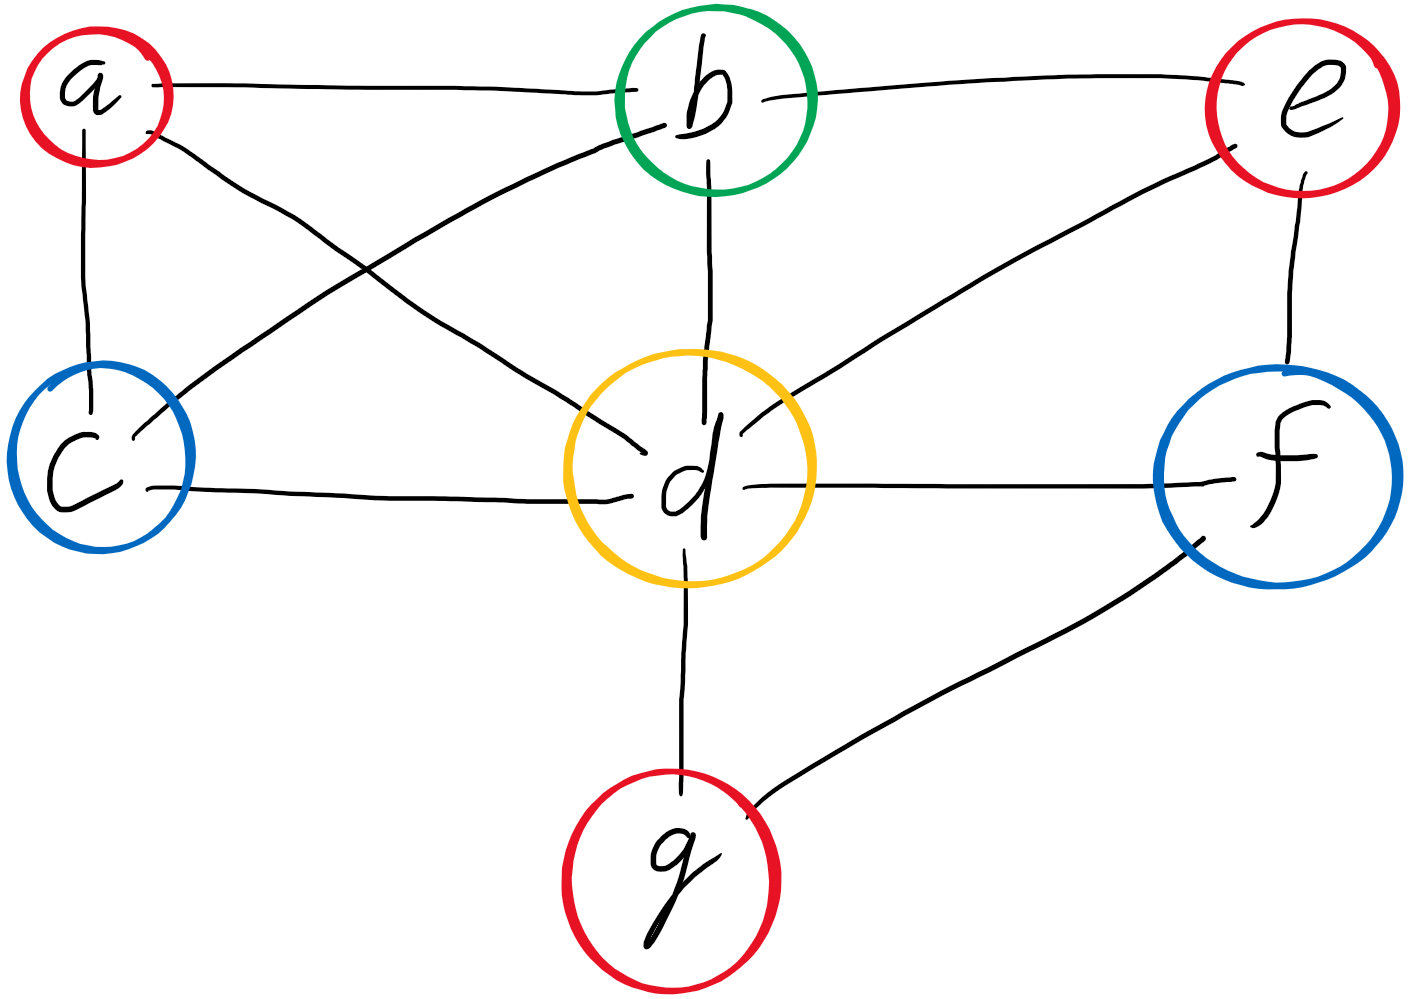
\includegraphics[width=0.5\textwidth]{img/4times.png}}

Это решение соответствует правильной раскраске графа. Если каждый цвет сопоставить одному из временных интервалов - комбинация цвета/времени и групп этого цвета будет решением.

\textbf{Ответ: Да, получится провести собрания в пятницу. Потребуется минимум 4 слота.}

\z Напомним, что граф называется двудольным, если его можно правильно раскрасить в два цвета.\\
{\bf а)}  Какое наибольшее число ребер может быть в простом двудольном графе на $k$ белых и $m$ чёрных вершинах? (В нем не должно быть ребер, соединяющих вершины одинакового цвета.)\\
\textbf{Решение:} \\
Для каждой из из белых вершин - максимальная возможная степень вершины будет равна $m$, если она соединена со всеми черными вершинами.
$$\sum_{v_i \in {white}} {deg(v_i)} = k \times m = |E|$$

\textbf{Ответ: $k\times m$ ребер }\\
{\bf б)} Какое наибольшее количество рёбер может быть в двудольном графе на $2n$ вершинах?
\textbf{Решение:} \\
Положим, белых вершин у нас $x$, тогда черных - $2n-x$. Тогда максимальное число ребер в этом графе - $x(2n-x)$.

Рассмотрим функцию $f(x) = x(2n-x)$. Для уравнения $x(2n-x) = 0$ есть 2 корня: 
$$\begin{cases} x_1 = 0 \\ x_2 =2n\end{cases}$$
Максимум для параболы достигается между корнями, для $x=n$:

$$max\{x(2n-x)\} = n^2; x = n$$

$\Rightarrow$ в двудольном графе на $2n$ вершинах максимум ребер будет при делении графа на 2 части по $n$ вершин. И число ребер равно $n^2$.

\textbf{Ответ: $n^2$}

\z Рассмотрим алфавит, состоящий только из двух букв $a$ и $b$. Все возможные слова, которые можно получить в этом алфавите, назовем языком.\\
{\bf a)} Докажите, что в этом языке можно составить слово, в котором любая трехбуквенная комбинация этих двух букв ($aaa$, $aab$, \ldots, $bba$, $bbb$) встречается ровно один раз.\\

\textbf{Решение:} \\
\centerline{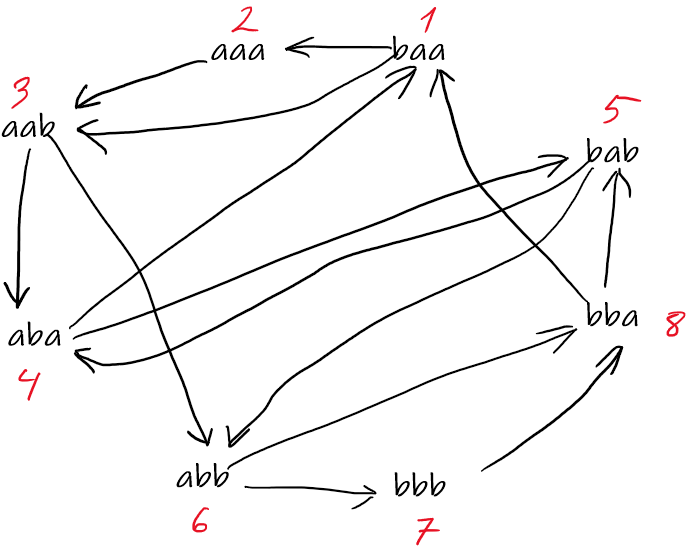
\includegraphics[width=0.5\textwidth]{img/letters.png}}

Составим граф $G$, вершинами которого будут все слова длины 3. Соединим ориентированным ребром два слова $w_1$ и $w_2$, если последние две буквы $w_1$ совпадают с первыми двумя буквами $w_2$

Если слова соединены ребром, то их можно написать подряд с пересечением последних двух и первых двух букв (baa → aaa дает слово baaa). Таким образом, путь образует слово, в котором поочередно идут комбинации трех букв, соответствующие вершинам этого пути.

Тогда слову, в котором любая комбинация из трех букв встречается ровно один раз, соответствует путь, проходящий по всем вершинам ровно один раз.

Таким путем является, например, путь по вершинами в порядке их нумерации от 1 до 8. 

Этот путь также оказался гамильтоновым циклом, поэтому можно составить такое слово, начиная с любой из трехбуквенных комбинаций.

\textbf{Ответ: Можно. Слово $baaababbba$ } \\
{\bf б)} Существует ли слово, которое удовлетворяет условию предыдущего пункта и начинается на $abba$? Если существует, то укажите его. Если не существует, то объясните, почему это невозможно.

\textbf{Решение:} \\
Так как мы начали наше слово на $abba$, в нем уже использована комбинация букв $abb$. Так как комбинация $bbb$ может идти только после $abb$, то в слове начинающемся на $abba$ будет дважды присутствовать как минимум комбинация $abb$ $\Rightarrow$ нельзя составить слово с началом на $abba$ в котором любая трехбуквенная комбинация встречается ровно один раз.

\textbf{Ответ: Не существует.}
\end{document}